%%%%%%%%%%%%%%%%%%%%%%%%%%%%%%%%%%%%%%%%%%%%%%%%%%%%%%%%%%%%%%%

% Set up document

\documentclass{beamer}
\usecolortheme{whale}
\setbeamersize{text margin left=5mm,text margin right=5mm}

% Used to create a section slide between section
\AtBeginSection[]{
  \begin{frame}
  \vfill
  \centering
  \begin{beamercolorbox}[sep=8pt,center,shadow=true,rounded=true]{title}
    \usebeamerfont{title}\insertsectionhead\par%
  \end{beamercolorbox}
  \vfill
  \end{frame}
}

% Remove default navigation symbols and add just  page number
\setbeamertemplate{navigation symbols}{} % Clear default navigation
\addtobeamertemplate{navigation symbols}{}{%
    \usebeamerfont{footline}%
    \usebeamercolor[fg]{footline}%
    \hspace{1em}%
    \insertframenumber/\inserttotalframenumber
}

% Used to create a section slide between section
\AtBeginSection[]{
  \begin{frame}[noframenumbering, plain]
  \vfill
  \centering
  \begin{beamercolorbox}[sep=8pt,center,shadow=true,rounded=true]{title}
    \usebeamerfont{title}\insertsectionhead\par%
  \end{beamercolorbox}
  \vfill
  \end{frame}
}


%%%%%%%%%%%%%%%%%%%%%%%%%%%%%%%%%%%%%%%%%%%%%%%%%%%%%%%%%%%%%%%

% Title page

\title{Stroke Audit Machine Learning (SAMueL)}
\subtitle{Investigating variation in clinical decision-making with explainable AI}


\author{Michael Allen\inst{1}, Kerry Pearn\inst{1}, Anna Laws\inst{1}, Keira Pratt-Boyden\inst{1}, Peter McMeekin\inst{3}, Martin James\inst{1,2} }
\institute{\inst{1} University of Exeter Medical School \inst{2} Royal Devon University Healthcare NHS Foundation Trust, and the Sentinel Stroke National Audit Programme (SSNAP) \inst{3} Northumbria University}

%\institute{Overleaf}
\date{December 2022}

%%%%%%%%%%%%%%%%%%%%%%%%%%%%%%%%%%%%%%%%%%%%%%%%%%%%%%%%%%%%%%%


\begin{document}

\begin{frame}
\titlepage
\end{frame}

%%%%%%%%%%%%%%%%%%%%%%%%%%%%%%%%%%%%%%%%%%%%%%%%%%%%%%%%%%%%%%%

\section{About us}

%%%%%%%%%%%%%%%%%%%%%%%%%%%%%%%%%%%%%%%%%%%%%%%%%%%%%%%%%%%%%%%

\begin{frame}{Who are we?}

\begin{itemize}
    \setlength{\itemsep}{3mm}
    \item We are modellers, data scientists, and qualitative researchers, based at the University of Exeter and Northumbria university.
    \item We work almost exclusively on the emergency stroke pathway (about the first 12 hours after stroke onset).
    \item We have worked extensively with the NHS on planning of emergency stroke services:

    \begin{itemize}
        \item We have worked on informing the number and location of \emph{thrombolysis} and \emph{thrombectomy} centres for NHS England, NHS Scotland, NHS Wales, NHS Northern Ireland, and including bespoke modelling for NHS East of England.
    \end{itemize}

    \item We work closely with the Sentinel Stroke National Audit Programme (SSNAP)
     
\end{itemize}
\end{frame}


%%%%%%%%%%%%%%%%%%%%%%%%%%%%%%%%%%%%%%%%%%%%%%%%%%%%%%%%%%%%%%%

\begin{frame}{Our current main interests}

\begin{itemize}
\setlength{\itemsep}{2mm}
    \item Understanding the between-hospital variation in use of thrombolysis.
    \item Modelling outcome after stroke and treatment with thrombolysis/thrombectomy:
        \begin{itemize}
            \item Survival, disability (modified Rankin Scale), life expectancy, utility, QALY.
        \end{itemize}
    \item Modelling the pre-hospital stroke pathway (selection of patients likely to be suitable for thrombectomy), and how that will affect outcomes and patient flows (including potential destabilisation of the regional emergency stroke care system).
    \item Modelling the potential impact of \emph{Mobile Stroke Units}, especially on whether they are likely to improve or worsen equity of access to emergency stroke care.
    \item Geographic modelling (as needed).
\end{itemize}
\end{frame}

%%%%%%%%%%%%%%%%%%%%%%%%%%%%%%%%%%%%%%%%%%%%%%%%%%%%%%%%%%%%%%%

\section{Geographic modelling}

%%%%%%%%%%%%%%%%%%%%%%%%%%%%%%%%%%%%%%%%%%%%%%%%%%%%%%%%%%%%%%%
\begin{frame}
\frametitle{Treatments for stroke}

\begin{columns}[t]
    \column{0.5\textwidth}
    \footnotesize{\textbf{Thrombolysis} aims to break down a clot by activating the body's own clot breakdown mechanisms.}
    
    \vspace{3mm}
    
    \footnotesize{Thrombolysis is given as an injection followed by an infusion (\emph{drip}).}
    
    \vspace{3mm}
    
    \footnotesize{Thrombolysis is available at all hospitals routinely admitting emergency stroke patients.} 
    
    \begin{center}
    \includegraphics[width=0.6\textwidth]{./images/thrombolysis_mechanism}
    \end{center}
    
    \column{0.5\textwidth}
    \footnotesize{\textbf{Thrombectomy} physically removes the clot.}
    
    \vspace{3mm}
    
    \footnotesize{Thrombectomy uses a mesh clot removal device guided under a CT scanner by a specialist operator.}
    
    \vspace{3mm}
    
    \footnotesize{Thrombectomy is only available at specialist centres} 
    
    \begin{center}
    \includegraphics[width=0.5\textwidth]{./images/thrombectomy_mesh}
    \end{center}

\end{columns}

\vspace{3mm}
\footnotesize{Both treatments are time-critical and lose effectiveness over the first hours after a stroke.}

\vspace{3mm}
\footnotesize{Note: Thrombolysis is often the \emph{gateway} to thrombectomy. Without local thrombolysis, a patient will often not be considered for thrombectomy.}



\end{frame}

%%%%%%%%%%%%%%%%%%%%%%%%%%%%%%%%%%%%%%%%%%%%%%%%%%%%%%%%%%%%%%%

\begin{frame}{Example of the challenges of geography in emergency stroke care}

\begin{columns}
    \begin{column}{0.5\textwidth}
        \begin{center}
        Time to thrombolysis\\   
        \vspace{3mm}
        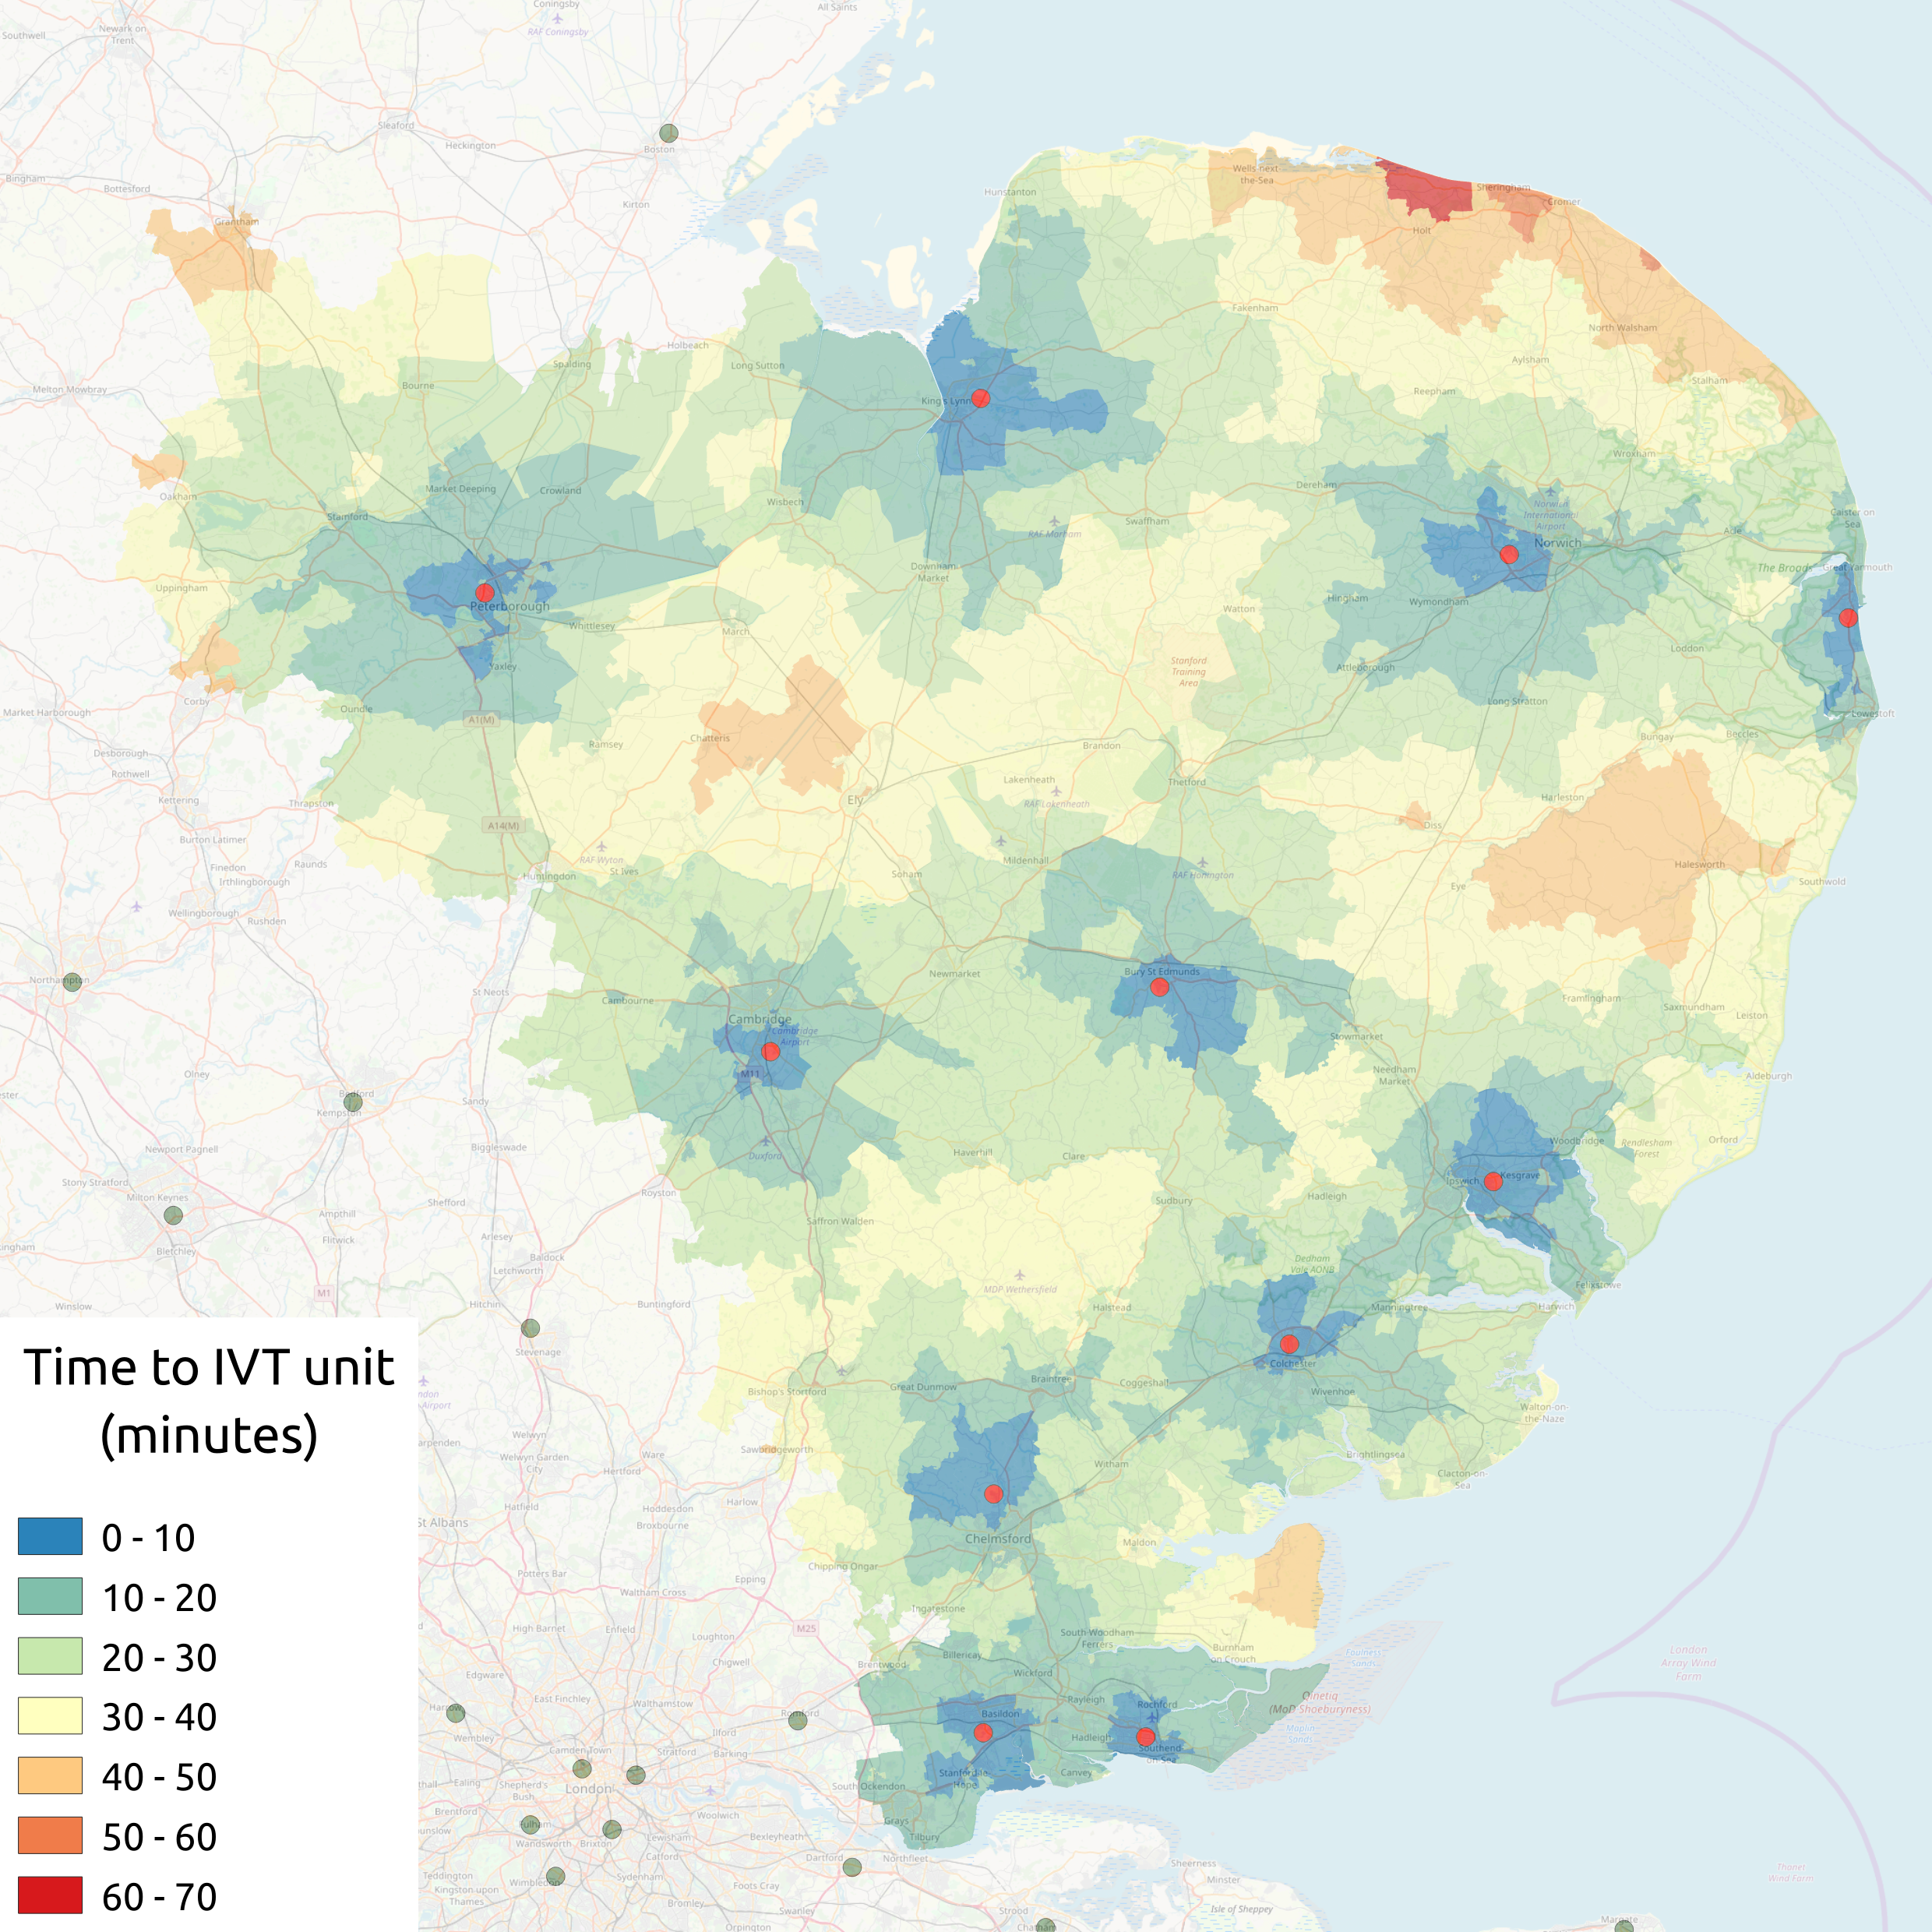
\includegraphics[width=0.95\textwidth]{./images/ivt_time_base}
        \end{center}        
    \end{column}
    
    \begin{column}{0.5\textwidth}
        \begin{center}
        Time to thrombectomy\\     
        \vspace{3mm}
        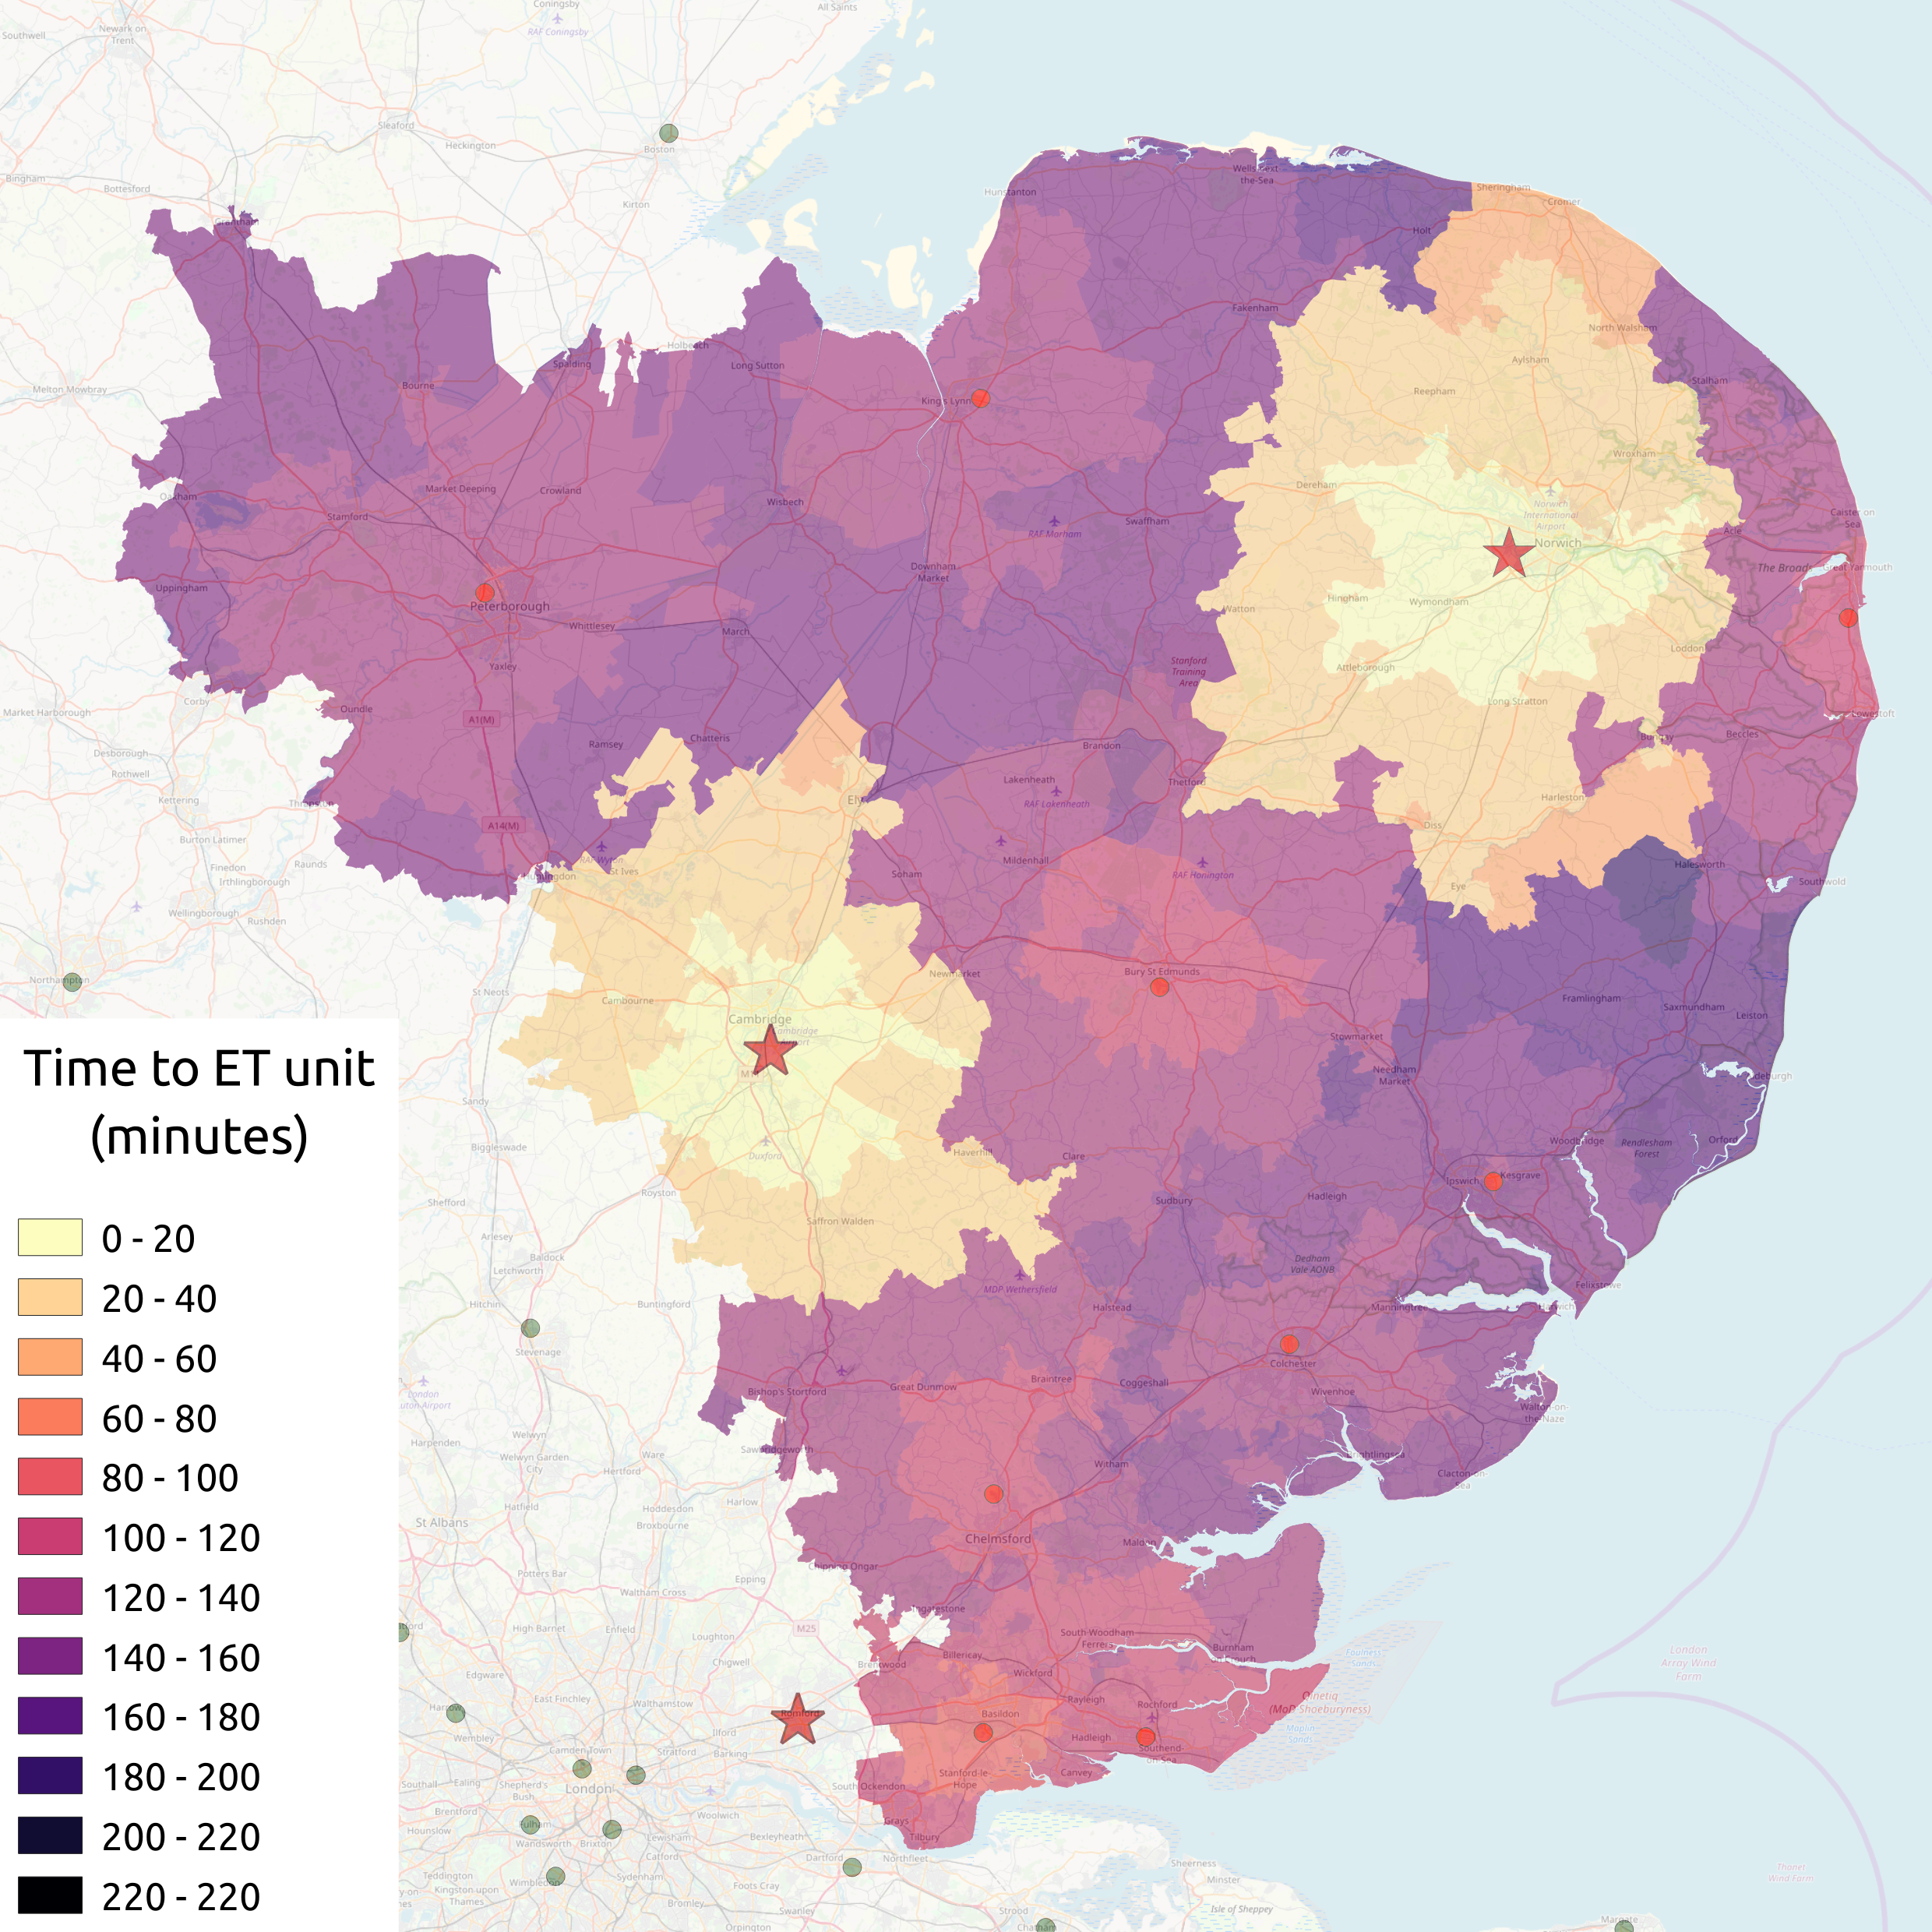
\includegraphics[width=0.95\textwidth]{./images/et_time_2et}
        \end{center}   
    
    \end{column}
\end{columns}
\end{frame}

%%%%%%%%%%%%%%%%%%%%%%%%%%%%%%%%%%%%%%%%%%%%%%%%%%%%%%%%%%%%%%%

\begin{frame}{And the impact on patient outcomes...}
\begin{footnotesize}
    


\begin{columns}[b]
    \begin{column}{0.5\textwidth}
        \begin{center}
        Outcome with modelled provision in 2018\\
        \vspace{3mm}
        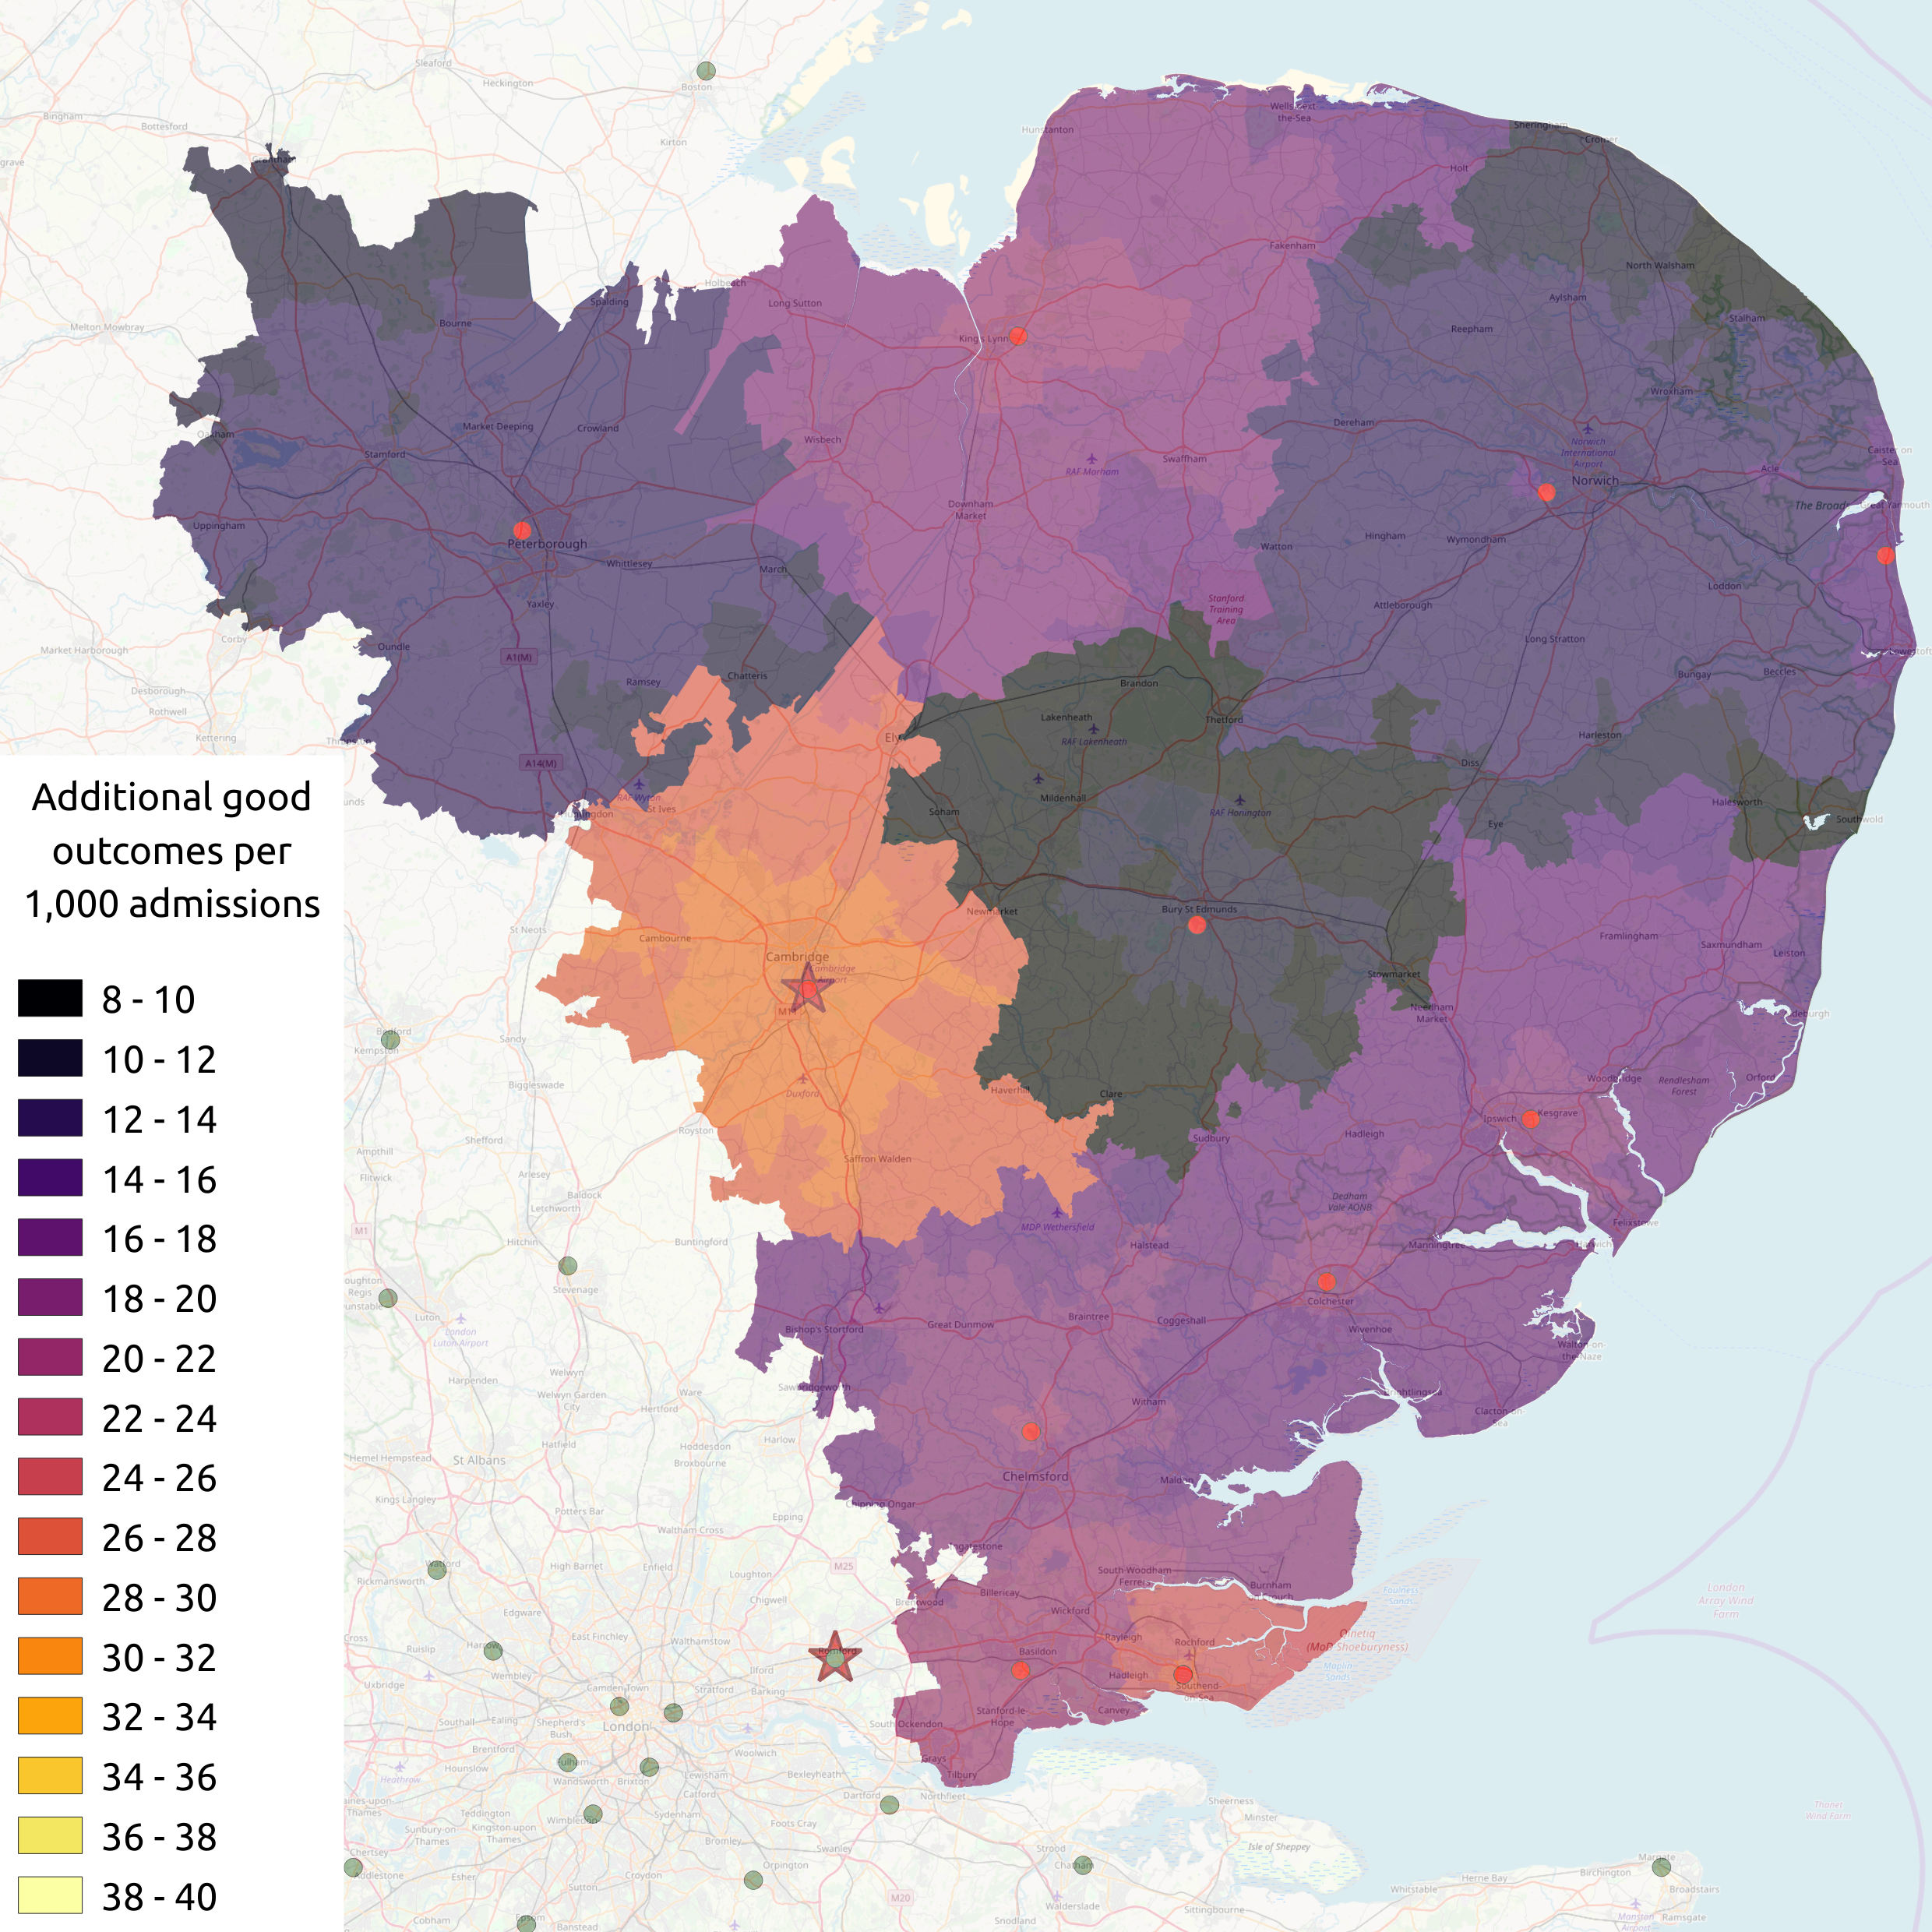
\includegraphics[width=0.95\textwidth]{./images/outcome_current_ivt_et}
        \end{center}        
    \end{column}
    
    \begin{column}{0.5\textwidth}
        \begin{center}
        Outcome if 20\% patients thrombolysed and region has two thrombectomy centres\\        
        \vspace{3mm}
        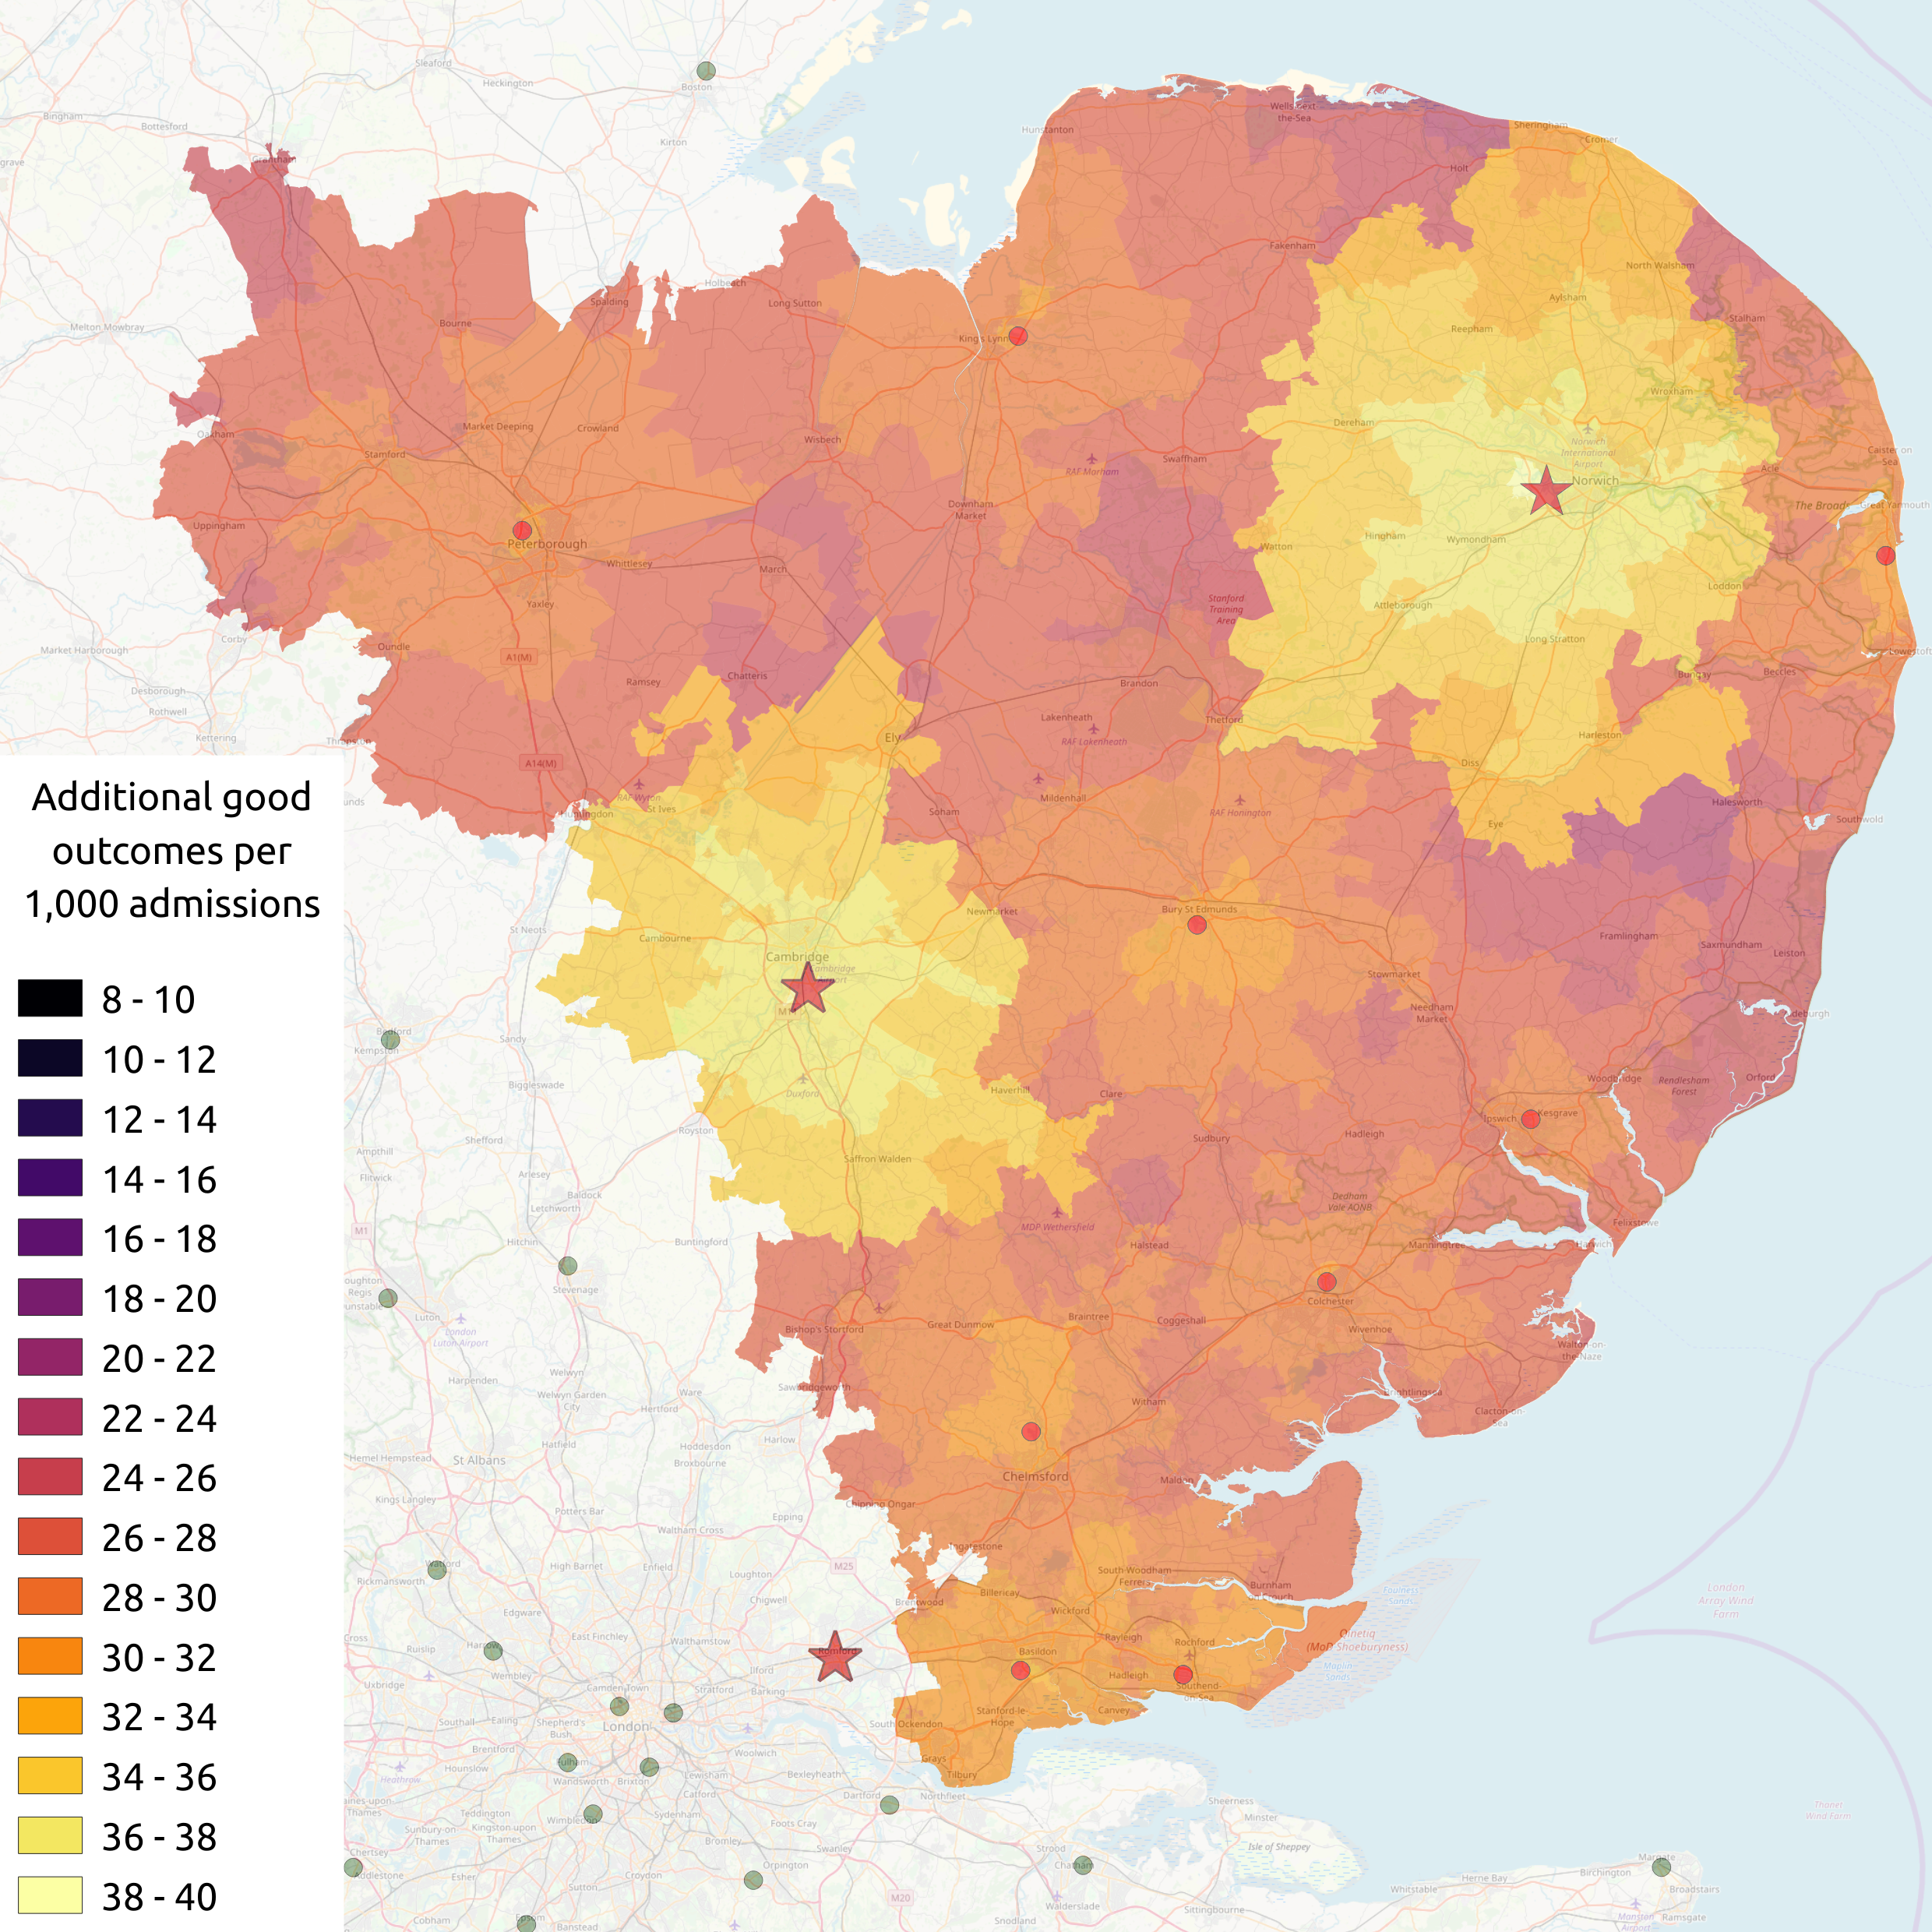
\includegraphics[width=0.95\textwidth]{./images/outcome_2et}
        \end{center}   
    
    \end{column}
\end{columns}

\vspace{3mm}
Since our earlier work, Peterborough has significantly improved use of thrombolysis, which also enables more patients to be considered for thrombectomy at Cambridge.

\end{footnotesize}
\end{frame}

%%%%%%%%%%%%%%%%%%%%%%%%%%%%%%%%%%%%%%%%%%%%%%%%%%%%%%%%%%%%%%%

\section{Clinical pathway modelling and machine learning}

%%%%%%%%%%%%%%%%%%%%%%%%%%%%%%%%%%%%%%%%%%%%%%%%%%%%%%%%%%%%%%%

\begin{frame}{Why does use of thrombolysis vary so much between hospitals, and why is it so short of the NHS target?}

\begin{center}
    \includegraphics[width=0.80\textwidth]{./images/thrombolysis_by_hospital}
\end{center}


\end{frame}


%%%%%%%%%%%%%%%%%%%%%%%%%%%%%%%%%%%%%%%%%%%%%%%%%%%%%%%%%%%%%%%

\begin{frame}
\frametitle{Breaking down the emergency stroke pathway into key steps}
\begin{center}
\includegraphics[width=1.0\textwidth]{./images/pathway}
\end{center}
We can model key changes to pathway:
\begin{small}

\begin{itemize}
    \item What if the pathway were faster?
    \item What if hospital determined the stroke onset time in more patients?
    \item What if clinical decision-making was like that of \emph{benchmark} hospitals? (Predict what treatment a patient would receive at other hospitals).
\end{itemize}
\end{small}
\footnotesize{We model these changes with a hospital's own patient population, to allow for inter-hospital variation in patient population characteristics.}
\end{frame}


%%%%%%%%%%%%%%%%%%%%%%%%%%%%%%%%%%%%%%%%%%%%%%%%%%%%%%%%%%%%%%%

\begin{frame}
\frametitle{Learning clinical decision making at each hospital}
\begin{itemize}
    \item By using machine learning, we are are able to predict what treatment any patient would likely receive at any hospital.
    \item We may then ask \emph{"What treatment would this patient receive at another hospital?"}
\end{itemize}

\begin{center}
\includegraphics[width=1.0\textwidth]{./images/ml_model_high_level}
\end{center}

\end{frame}


%%%%%%%%%%%%%%%%%%%%%%%%%%%%%%%%%%%%%%%%%%%%%%%%%%%%%%%%%%%%%%%

\section{Skipping a lot of work ......}

%%%%%%%%%%%%%%%%%%%%%%%%%%%%%%%%%%%%%%%%%%%%%%%%%%%%%%%%%%%%%%%

\begin{frame}{Why do hospitals differ so much in use of thrombolysis?}

Though differences in patient population explain some of the differences in thrombolysis use (and so units should not all have the same expected thrombolysis use), hospitals also differ in their willingness to use thrombolysis.

\vspace{3mm}

All hospitals would give thrombolysis to this patient:
\begin{itemize}
\begin{footnotesize}
    \item Onset to arrival = 80 mins
    \item Arrival to scan = 20 mins
    \item Moderate-to-severe stroke (NIHSS = 15)
    \item No prior disability level 
    \item Onset time is known precisely
\end{footnotesize}
\end{itemize}

\vspace{3mm}

But only 6 out of 10 hospitals would give thrombolysis to the same patient except them having an estimated stroke onset time and a mild pre-stroke disability (able to look after themselves, but unable to do all of their previous activities).

\end{frame}

%%%%%%%%%%%%%%%%%%%%%%%%%%%%%%%%%%%%%%%%%%%%%%%%%%%%%%%%%%%%%%%

\section{Why are we here?}

%%%%%%%%%%%%%%%%%%%%%%%%%%%%%%%%%%%%%%%%%%%%%%%%%%%%%%%%%%%%%%%

\begin{frame}{Why are we here?}

\begin{itemize}
    \setlength{\itemsep}{5mm}
    
    \item We want our work to have the best impact for patients.
    
    \item We are looking for teams that we can share our work with (in the early stages) so that we can use the feedback to refine our work.

    \item You get some (hopefully!) useful analysis, and we get to improve how we share our analysis.

\end{itemize}
\end{frame}

\end{document}

